\section{用户使用手册}
\subsection{基础功能}
\subsubsection{开启程序}
点击王者荣耀连连看文件中的code.exe开启游戏,进入菜单界面如图\ref{fig:usemain}。

\subsubsection{开始游戏}
在菜单界面中点击开始游戏,进入游戏界面如图\ref{fig:play}所示,左边游戏区域为练练看游戏,右边设置区域可以查看游戏分数和剩余游戏时间。具体说明如下:
\begin{enumerate}
    \item 一次消除获得2分,相邻两次消除时间小于2s会有加倍得分;
    \item 普通游戏玩家点击提示会消除一对图片,VIP玩家会消除多对;
    \item 点击洗牌会对图片随机排序;
    \item 点击退出返回到主界面。
\end{enumerate}

\subsubsection{游戏设置}
在菜单界面点击游戏设计,进入游戏设置界面如图\ref{fig:setting2}所示,可选择游戏难度,即游戏人物数量,默认为13个英雄。对应地,游戏难度越高,连续消除的额外得分也越高。
\begin{figure}[!htbp]
    % \begin{figure}[H]
        \centering
        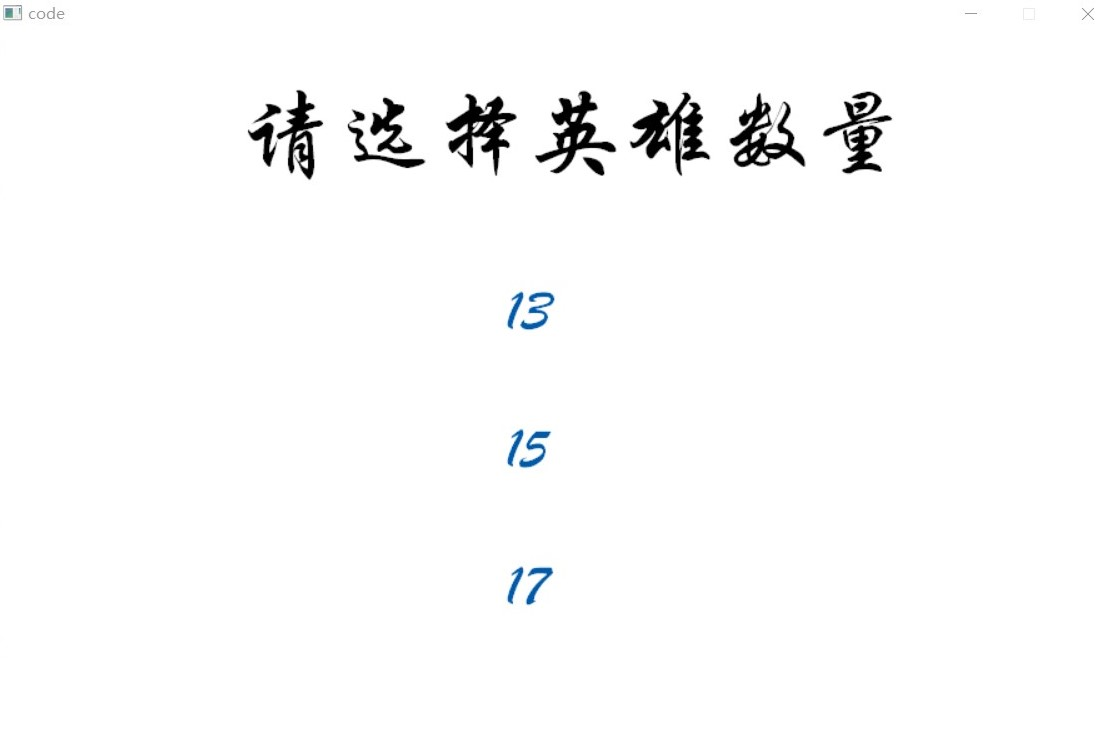
\includegraphics[width=0.6\textwidth]{setting.jpg}
        \caption{游戏设置界面} \label{fig:setting2}
\end{figure}

\subsubsection{游戏排名}
在菜单界面点击游戏设计,进入游戏设置界面如图\ref{fig:rank2}所示。
\begin{figure}[!htbp]
    % \begin{figure}[H]
        \centering
        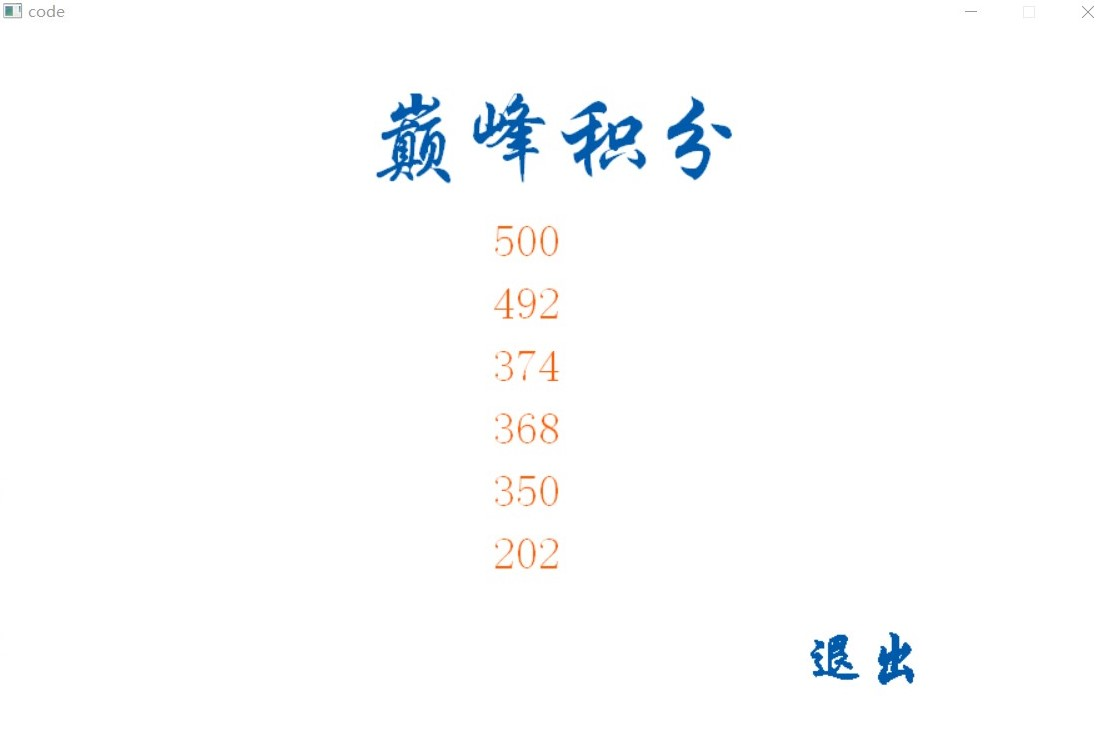
\includegraphics[width=0.6\textwidth]{rank.jpg}
        \caption{游戏排名界面} \label{fig:rank2}
\end{figure}

\subsubsection{游戏充值}
在菜单界面点击充值,游戏中基础得分100分,英雄获得全皮肤,点击提示有多对消除。再次点击退款可能回到普通模式。

\subsection{扩展功能}
用户可替换./fig文件夹中的图片,定制属于自己的练练看。注意图片总数和命名不能改变。
